\documentclass{article}

\usepackage{amsmath}
\usepackage{amsfonts}
\usepackage{amssymb}
\usepackage{multicol}
\usepackage{wrapfig}
\usepackage{mathenv}
\usepackage{multirow}
\usepackage{enumerate}

\usepackage{vmargin}
\setmarginsrb{2.5cm}{2.5cm}{2.5cm}{2.9cm}{0cm}{0cm}{0cm}{0cm}

\usepackage[utf8]{inputenc}

\usepackage[french]{babel}
\selectlanguage{french}

\usepackage{color}
\usepackage{hyperref}
\hypersetup{pdfborder={0 0 0}, colorlinks=true, urlcolor=blue, linkcolor = darkred}
\usepackage{graphicx}
\graphicspath{{graphsEx3/}} 
\usepackage{listings}
\definecolor{colKeys}{rgb}{0.75,0,0}
\definecolor{colIdentifier}{rgb}{0,0,0}
\definecolor{colComments}{rgb}{0.75,0.75,0}
\definecolor{colString}{rgb}{0,0,0.7}

\usepackage{verbatim}
\usepackage{moreverb}

\lstset{
basicstyle=\ttfamily\small, %
identifierstyle=\color{colIdentifier}, %
keywordstyle=\color{colKeys}, %
stringstyle=\color{colString}, %
commentstyle=\color{colComments}, %
showspaces=false,
}
\lstset{language=java}

% Commandes personnelles %

\definecolor{darkred}{rgb}{0.85,0,0}
\definecolor{darkblue}{rgb}{0,0,0.7}
\definecolor{darkgreen}{rgb}{0,0.6,0}
\definecolor{darko}{rgb}{0.93,0.43,0}
\definecolor{maintitle}{rgb}{0.66,0,0.22}
\definecolor{title}{rgb}{0,0.5,0.5}
\definecolor{quote}{rgb}{0.7,0.7,0.7}
\definecolor{forestgreen}{rgb}{0.14,0.54,0.13}
\definecolor{cyan4}{rgb}{0,0.54,0.54}
\definecolor{firebrick4}{rgb}{0.54,0.1,0.1}
\newcommand{\maintitlecolor}[1]{\textcolor{maintitle}{#1}}
\newcommand{\titre}[1]{\textcolor{title}{#1}}
\newcommand{\tsect}[1]{\titre{\section{#1}}}
\newcommand{\tssect}[1]{\titre{\subsection{#1}}}
\newcommand{\tsssect}[1]{\titre{\subsubsection{#1}}}
\newcommand{\vect}[1]{\overrightarrow{#1}}
\newcommand{\dred}[1]{\textcolor{darkred}{\textbf{#1}}}
\newcommand{\dgre}[1]{\textcolor{darkgreen}{\textbf{#1}}}
\newcommand{\dblu}[1]{\textcolor{darkblue}{\textbf{#1}}}
\newcommand{\dora}[1]{\textcolor{darko}{\textbf{#1}}}
\newcommand{\gre}[1]{\textcolor{darkgreen}{#1}}
\newcommand{\blu}[1]{\textcolor{darkblue}{#1}}
\newcommand{\ora}[1]{\textcolor{darko}{#1}}
\newcommand{\rouge}[1]{\textcolor{darkred}{#1}}
\newcommand{\quotecolor}[1]{\textcolor{quote}{#1}}
\newcommand{\forest}[1]{\textcolor{forestgreen}{#1}}
\newcommand{\cyan}[1]{\textcolor{cyan4}{#1}}
\newcommand{\firebrick}[1]{\textcolor{firebrick4}{#1}}
\newcommand{\ceil}[1]{\left\lceil #1 \right\rceil}
\newcommand{\cdil}[1]{\left\lfloor #1 \right\rfloor}
\newcommand{\term}[1]{\textit{\textcolor{maintitle}{#1}}}
\newcommand{\image}[1]{\includegraphics{#1}}
\newcommand{\imageR}[2]{\includegraphics[width=#2px]{#1}}
\newcommand{\imageRT}[2]{\includegraphics[height=#2px]{#1}}
\newcommand{\img}[1]{\begin{center}\includegraphics[width=400px]{#1}\end{center}}
\newcommand{\imag}[1]{\begin{center}\includegraphics{#1}\end{center}}
\newcommand{\imgR}[2]{\begin{center}\includegraphics[width=#2px]{#1}\end{center}}
\newcommand{\imgRT}[2]{\begin{center}\includegraphics[height=#2px]{#1}\end{center}}
\newcommand{\point}[2]{\item \ora{\underline{#1}} : \textit{#2}}
\newcommand{\bfp}[2]{\item \textbf{#1} : \textit{#2}}
\newcommand{\sumparam}[3]{\sideset{}{_{#1}^{#2}}\sum{#3}}
\newcommand{\sumin}[3]{\sideset{}{_{i=#1}^{#2}}\sum{#3}}
\newcommand{\sumkn}[3]{\sideset{}{_{k=#1}^{#2}}\sum{#3}}
\newcommand{\intin}[3]{\sideset{}{_{#1}^{#2}}\int{#3}}
\newcommand{\stitre}[1]{\noindent\textbf{\underline{#1}} \\}
\newcommand{\R}{\mathbb{R}}
\newcommand{\Z}{\mathbb{Z}}
\newcommand{\N}{\mathbb{N}}
\newcommand{\ualpha}{\vect{u_\alpha}}
\newcommand{\valpha}{\vect{v_\alpha}}
\newcommand{\palpha}{\vect{\Psi_\alpha}}
\newcommand{\npcomp}{\term{$\mathcal{NP}$-complet}}
\newcommand{\npcompl}{\term{$\mathcal{NP}$-complet} }
\DeclareMathAlphabet{\mathpzc}{OT1}{pzc}{m}{it}
\newtheorem{de}{D\'efinition}[section]
\newtheorem{rap}{Rappel}
\newtheorem{proof}{Preuve}
\newtheorem{note}{Note}[section]
\newtheorem{propriete}{Propri\'et\'e}[section]
\newtheorem{exemple}{Exemple}[section]
\newtheorem{corollaire}{Corollaire}[section]
\newtheorem{rem}{Remarque}[section]
\newtheorem{rems}{Remarques}[section]
\newtheorem{thm}{Th\'eor\`eme}[section]
\newtheorem{illustration}{Illustration}[section]
\newtheorem{pbm}{Problème}[section]
\newenvironment{pblm}{\hbox{\raisebox{0.4em}{\vrule depth 1pt height 0.4pt width 5cm}}\begin{pbm}}
{\end{pbm}\hbox{\raisebox{0.4em}{\vrule depth 1pt height 0.4pt width 5cm}}}
\newenvironment{demonstration}{\begin{proof}[\textnormal{\textbf{Preuve.}}]}{\end{proof}}

\begin{sffamily}
\title{$ $ \\ $ $ \\$ $\\$ $\\$ $\\$ $ \\$ $\\$ $\\
\begin{Huge}\maintitlecolor{Intelligence Artificielle}\end{Huge} \\ 
$ $ \\ 
\begin{LARGE}\textit{Devoir 3}\end{LARGE}}
\author{\textit{Xavier Dubuc} \\ MA1 Info \\ \url{xavier.dubuc@umons.ac.be} \\$ $ \\$ $\\$ $\\
\hbox{\raisebox{0.4em}{\vrule depth 1pt height 0.4pt width 5cm}} \\ $ $\\$ $ \\$ $\\$ $\\$ $\\$ $\\$ $\\$ $\\
$ $\\$ $ \\$ $\\$ $\\

\includegraphics[scale=0.3]{UMONS.pdf}$\qquad \qquad$
\includegraphics[scale=0.1]{faculte.pdf}}
%\date{}
\end{sffamily}

\begin{document}\begin{sffamily}

\maketitle

\newpage

\noindent \textbf{Question.} \textit{Supposons qu’un langage en logique du premier ordre soit défini à partir du vocabulaire 
suivant :} 
\textit{\begin{itemize}
\item quatre symboles constants : 0, 3, 7 et 9;
\item un prédicat binaire $\leq(x, y)$ (que l’on écrira ''$x \leq y$");
\item une fonction binaire $+(x, y)$ (que l’on écrira ''$x + y$").
\end{itemize}}

\noindent \textit{Supposons également qu’une base de connaissance KB contiennent les huit axiomes suivants :}
\begin{enumerate}
\item $0 \leq 3$.
\item $7 \leq 9$.
\item $\forall x,\ x \leq x$.
\item $\forall x,\ x \leq x + 0$.
\item $\forall x,\ x + 0 \leq x$.
\item $\forall x, y,\ x + y \leq y + x$.
\item $\forall w, x, y, z,\ w \leq y \wedge x \leq z \Rightarrow w + x \leq y + z$.
\item $\forall x, y, z,\ x \leq y \wedge y \leq z \Rightarrow x \leq z$.
\end{enumerate}

\noindent \textit{En ne vous basant que sur la connaissance décrite ci-dessus,}
\begin{enumerate}
\item[a)] \textit{donnez une preuve de type ''backward chaining" de la phrase ''$7 \leq 3 + 9$".}\\

L'idée de la preuve est de partir de l'objectif et de vérifier les prémisses nécessaires pour que l'objectif soit vérifié, en 
essayant de se ramener à un axiome atomique de la \textbf{KB}. En agissant de la sorte, on va trouver une liste de prémisses de 
\textbf{KB} qui permettent d'inférer l'objectif.

\begin{proof}[Backward Chaining]$ $\\
\begin{enumerate}[1.]
\item On commence donc par l'objectif.
\begin{figure}[h!]
    \begin{center}
    \includegraphics[width=0.2\textwidth]{backward1.pdf}
    \caption{Backward : 1ère étape}
    \end{center}	
\end{figure}

\item On choisit les prémisses donnés par la règle $8.\  x, y, z,\ x \leq y \wedge y \leq z \Rightarrow x \leq z$.\\
En effet, si on choisit la substitution $\theta = \{x/7, y/(7+0), z/(9+3)\}$, on a : 
$$8_\theta := \forest{7 \leq (7+0)} \wedge \firebrick{(7+0) \leq (9+3)} \Rightarrow 7 \leq 9+3$$
Le \forest{premier prémisse} appartient à \textbf{KB}, on ne doit donc plus s'occuper que \firebrick{du second}.
\begin{figure}[h!]
    \begin{center}
    \includegraphics[width=0.3\textwidth]{backward2.pdf}
    \caption{Backward : 2ème étape}
    \end{center}	
\end{figure}

\item On choisit à nouveau les prémisses donnés par la règle $8^b.\ x_1, y_1, z,\ x_1 \leq y_1 \wedge y_1 \leq z 
\Rightarrow x_1 \leq z_1$.\\ La substitution $\theta$ devient : $$\theta = \{x/7, y/(7+0), z/(9+3), x_1/(7+0), y_1/(0+7)\}$$
et elle nous fournit :
$$8^b_\theta := \firebrick{(7+0)\leq (0+7)} \wedge \firebrick{(0+7)\leq (9+3)}$$
\newpage
\begin{figure}[h!]
    \begin{center}
    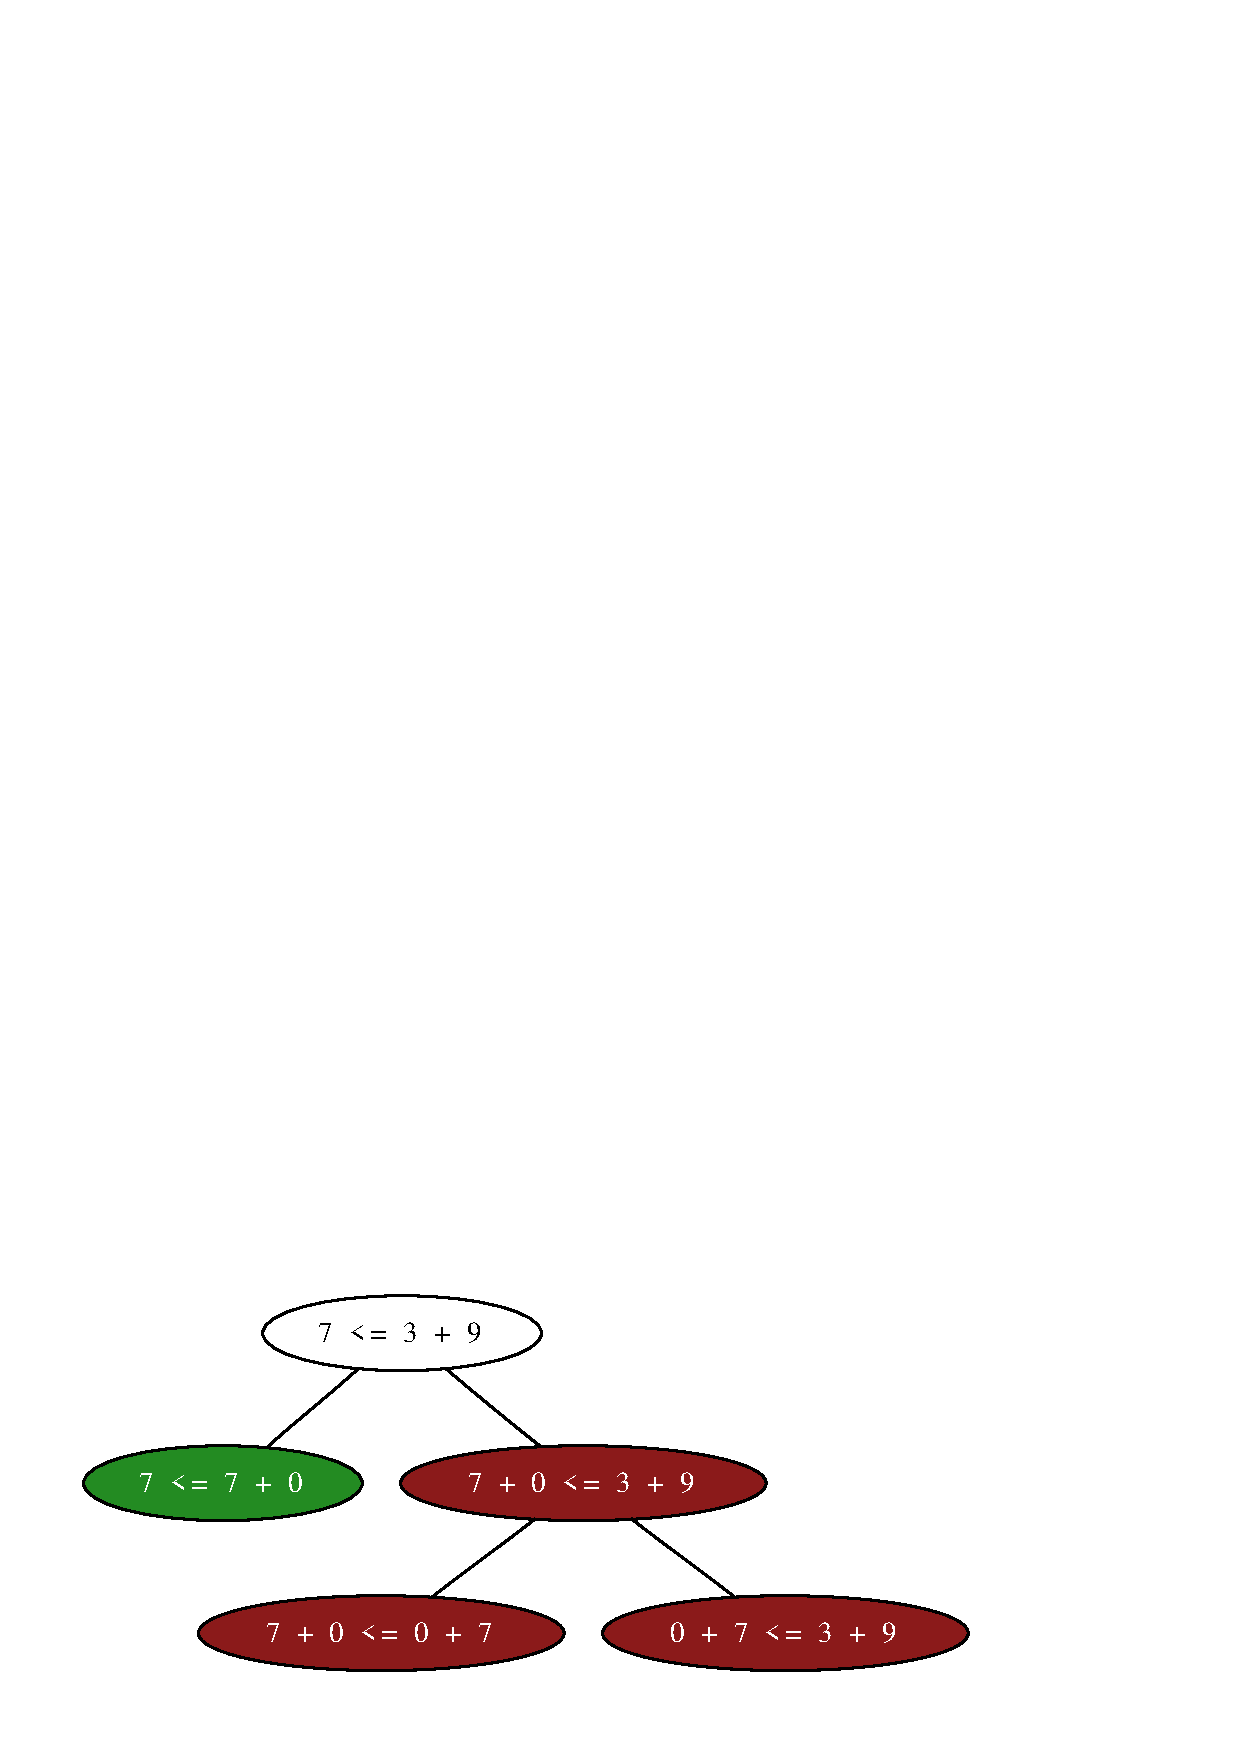
\includegraphics[width=0.5\textwidth]{backward3.pdf}
    \caption{Backward : 3ème étape}
    \end{center}	
\end{figure}
\begin{itemize}
\item Le premier prémisse est vérifié via la règle $6\ x_1, y_1,\ x_1 + y_1 \leq y_1 + x_1$ en appliquant $\theta$, en 
effet on obtient : $$6_\theta := \forest{(7+0)\leq (0+7)}$$, ce prémisse appartient donc à \textbf{KB}.
\begin{figure}[h!]
    \begin{center}
    \includegraphics[width=0.5\textwidth]{backward4.pdf}
    \caption{Backward : 4ème étape}
    \end{center}	
\end{figure}
\item Le second prémisse est vérifié via la règle $7\ \forall w, x, y_2, z_2,\ w \leq y_2 \wedge x \leq z_2 \Rightarrow w + x 
\leq y_2 + z_2$ en ajoutant à $\theta$ les substitutions $\{y_2/3,z_2/9\}$. $\theta$ devient donc : 
$$ \theta = \{x/7, y/(7+0), z/(9+3), x_1/(7+0), y_1/(0+7), y_2/3, z_2/9\} $$ et elle nous fournit :
$$7_\theta := \forest{0\leq 3} \wedge \forest{7\leq 9} \Rightarrow 0+7\leq3+9$$
\begin{figure}[h!]
    \begin{center}
    \includegraphics[width=0.5\textwidth]{backward5.pdf}
    \caption{Backward : 5ème étape}
    \end{center}	
\end{figure}
\end{itemize}
Les 2 premisses restants sont des axiomes atomiques de \textbf{KB}, on a donc trouvé une substitution et une liste de prémisses 
permettant d'inférer notre objectif. On peut donc conclure que notre objectif est vérifié.
\begin{figure}[h!]
    \begin{center}
    \includegraphics[width=0.5\textwidth]{backward6.pdf}
    \caption{Backward : étape finale}
    \end{center}	
\end{figure}
\end{enumerate}
\begin{flushright}
$\square$
\end{flushright}
\end{proof}

\item[b)] \textit{donnez une preuve de type ''forward chaining" de la phrase ''$7 \leq 3 + 9$".}\\

L'idée de la preuve est de se baser sur les axiomes de la \textbf{KB} et d'inférer, via des applications du \textbf{Modus 
Ponens}, des nouveaux faits atomiques.
\begin{rap}[Modus Ponens]
$ $\\\fbox{
\begin{minipage}{0.9\textwidth}\begin{center}
Soit des phrases atomiques $p_i$, $p'_i$ et $q$; \\ ainsi qu'une substitution $\theta$ telle que $SUBST(\theta, p_i) = 
SUBST(\theta, p'_i)$ pour tout $i$.\\ Alors $p_1$, $p_2$, ..., $p_n$, $(p_1 \wedge p_2 \wedge ... \wedge p_n \Rightarrow q)\ 
SUBST(\theta, q)$.\end{center}\end{minipage}}
\end{rap}

\begin{proof}[Forward Chaining]$ $\\
\begin{enumerate}[1.]
\item On part des 2 axiomes atomiques $(0\leq 3)$ et $(7\leq 9)$.
\begin{figure}[h!]
    \begin{center}
    \includegraphics[width=0.35\textwidth]{forward1.pdf}
    \caption{Forward : 1ère étape}
    \end{center}	
\end{figure}

\item Soit la substitution $\theta = \{w/0,x/7,y/3,z/9\}$,\\
appliquons $\theta$ à la règle $7\ \forall w, x, y, z,\ w \leq y \wedge x \leq z \Rightarrow w + x \leq y + z$, \\
$\Rightarrow$ on infère de la sorte que $\boxed{(0+7)\leq (3+9)}$.
\begin{figure}[h!]
    \begin{center}
    \includegraphics[width=0.35\textwidth]{forward2.pdf}
    \caption{Forward : 2ème étape}
    \end{center}	
\end{figure}
\newpage
\item Soit la substitution $\theta_2 = \{x/(7+0), y/(0+7), z/(3+9), a/7, b/0\}$,\\
appliquons $\theta_2$ aux règles :
\begin{itemize}
\item $6.\ \forall a, b,\ a + b \leq b + a\ \blu{\Rightarrow 6_\theta := 7+0\leq 0+7}$,
\item $8.\ \forall x, y, z,\ x \leq y \wedge y \leq z \Rightarrow x \leq z\ \blu{\Rightarrow 8_\theta := (7+0) \leq (0+7) \wedge 
(0+7) \leq (3+9) \Rightarrow (7+0) \leq (3+9)}$,
\end{itemize}
$\Rightarrow$ on infère de la sorte que $\boxed{(7+0)\leq (3+9)}$ 
\begin{figure}[h!]
    \begin{center}
    \includegraphics[width=0.5\textwidth]{forward3.pdf}
    \caption{Forward : 3ème étape}
    \end{center}	
\end{figure}

\item Finalement, en utilisant la substitution $\theta_3 = \{x/7, y/(7+0), z/(3+9)\}$,\\
appliquons $\theta_3$ aux règles : 
\begin{itemize}
\item $4.\ \forall x \leq x + 0\ \blu{\Rightarrow 4_\theta := 7 \leq 7+0}$,
\item $8.\ \forall x, y, z,\ x \leq y \wedge y \leq z \Rightarrow x \leq z\ \blu{\Rightarrow 8_\theta := 7 \leq (7+0) \wedge 
(7+0) \leq (3+9) \Rightarrow 7 \leq (3+9)}$,
\end{itemize}
$\Rightarrow$ on infère de la sorte que \forest{$\boxed{7\leq (3+9)}$}
\begin{figure}[h!]
    \begin{center}
    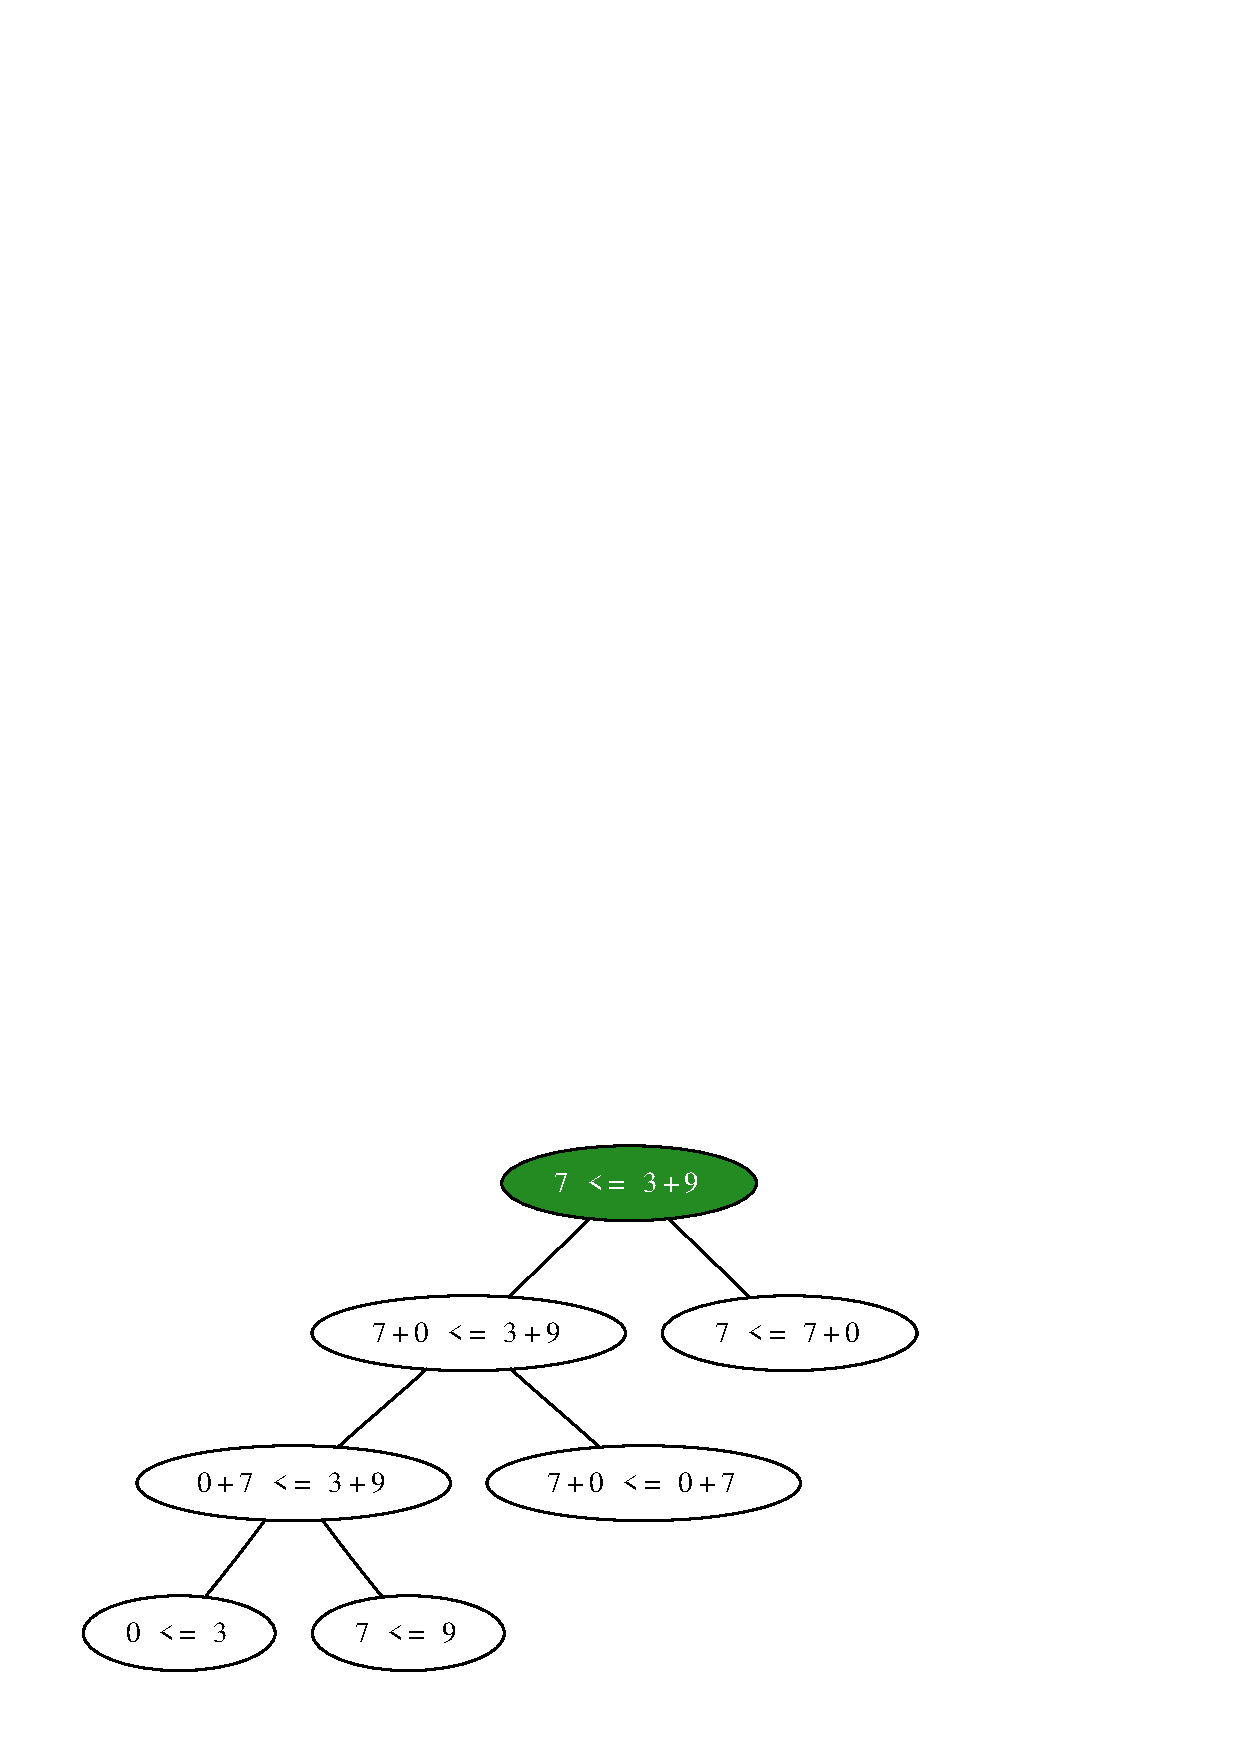
\includegraphics[scale=0.5]{forwardend.pdf}
    \caption{Forward : étape finale}
    \end{center}	
\end{figure}
\end{enumerate}
\begin{flushright}
$\square$
\end{flushright}
\end{proof}

\end{enumerate}

\end{sffamily}\end{document}